%!TeX root=../main.tex

\chapter{Resultados}
\label{cap:resultados}

Este capítulo apresenta os resultados obtidos durante o experimento, acompanhados de uma discussão sobre os dados coletados. Inicialmente, 
são analisadas as métricas de desempenho dos participantes, com o objetivo de avaliar o funcionamento do sistema de recomendação de 
exercícios e investigar  a contribuição da abordagem de ensino e das explicações fornecidas pela IA para o aprendizado. Em seguida, 
são apresentadas e discutidas as respostas ao questionário aplicado, buscando compreender a experiência dos participantes e identificar 
possíveis pontos de melhoria no sistema.

\section{Desempenho dos usuários}
\label{sec:users_performances}
Na Tabela~\ref{tab:piece_accuracy}, são apresentadas as taxas de acerto por peça em cada módulo, acompanhadas da quantidade de exercícios em que cada uma aparece.

Destaca-se a predominância do Peão entre os exercícios, o que pode ser explicado, principalmente, por sua maior quantidade no tabuleiro, aumentando a 
probabilidade de ser selecionado pelo gerador de questões. Em contrapartida, as peças promovidas aparecem com menor frequência, devido à sua menor disponibilidade 
nas posições utilizadas para a geração dos exercícios.

\begin{table}[H]
\centering
\caption{Taxa de acerto por peça}
\label{tab:piece_accuracy}
\small
\resizebox{\textwidth}{!}{%
\begin{tabular}{>{\centering\arraybackslash}m{1.2cm} >{\centering\arraybackslash}m{1.7cm} >{\centering\arraybackslash}m{1.7cm} >{\centering\arraybackslash}m{1.7cm} >{\centering\arraybackslash}m{1.7cm} >{\centering\arraybackslash}m{1.7cm} >{\centering\arraybackslash}m{1.7cm} >{\centering\arraybackslash}m{1.7cm}}
\toprule
Peça & \makecell{Reconhe-\\cimento} & Movimento 1 & Movimento 2 & Promoção & Drop & Xeque-mate & Total \\
\midrule
+B & 60.0\% (10) & 94.6\% (74) & 100.0\% (2) & — & — & 62.5\% (8) & 88.3\% (94) \\ \midrule
+L & 75.0\% (4) & 85.9\% (78) & — & — & — & 50.0\% (4) & 83.7\% (86) \\ \midrule
+N & 71.4\% (7) & 82.4\% (91) & — & — & — & — & 81.6\% (98) \\ \midrule
+P & 95.8\% (24) & 83.6\% (61) & 0.0\% (2) & — & — & 100.0\% (2) & 85.4\% (89) \\ \midrule
+R & 81.0\% (21) & 97.6\% (82) & 100.0\% (2) & — & — & 76.9\% (26) & 90.8\% (131) \\ \midrule
+S & 100.0\% (2) & 84.5\% (84) & — & — & — & — & 84.9\% (86) \\ \midrule
B & 88.4\% (43) & 96.8\% (63) & 96.7\% (30) & 91.1\% (235) & 95.7\% (188) & 54.5\% (11) & 92.6\% (570) \\ \midrule
G & 87.7\% (195) & 94.0\% (67) & 91.2\% (113) & — & 94.0\% (84) & 77.1\% (83) & 88.6\% (542) \\ \midrule
K & 87.3\% (110) & 97.3\% (74) & 98.6\% (70) & — & — & — & 93.3\% (254) \\ \midrule
L & 89.2\% (176) & 95.8\% (72) & 90.7\% (54) & 92.7\% (41) & 85.7\% (56) & 66.7\% (6) & 90.1\% (405) \\ \midrule
N & 95.7\% (185) & 93.8\% (65) & 100.0\% (36) & 97.3\% (113) & 80.2\% (81) & 71.4\% (7) & 93.2\% (487) \\ \midrule
P & 95.4\% (723) & 96.1\% (76) & 99.7\% (311) & 94.5\% (164) & 82.2\% (259) & 50.0\% (2) & 93.9\% (1535) \\ \midrule
R & 91.0\% (89) & 94.0\% (83) & 97.6\% (42) & 94.0\% (184) & 100.0\% (30) & 76.9\% (13) & 93.7\% (441) \\ \midrule
S & 85.5\% (186) & 88.9\% (72) & 88.0\% (100) & 88.0\% (75) & 94.4\% (72) & 87.5\% (8) & 88.1\% (513) \\
\bottomrule
\end{tabular}
}
\end{table}

Os gráficos do Apêndice~\ref{ap:modules_performances} apresentam a taxa de acerto de cada participante por módulo. Entretanto, como uma mesma lista pode conter 
exercícios de diferentes módulos, a quantidade de questões de cada tipo pode variar consideravelmente. Dessa forma, essa métrica deve ser interpretada com cautela, 
pois, quanto menor a quantidade de exercícios de determinado módulo, maior pode ser o impacto de uma única resposta incorreta sobre a taxa de acerto.

Os gráficos do Apêndice~\ref{ap:avg_response_time}, por sua vez, apresentam o tempo médio de resposta de cada participante por lista e módulo. De maneira geral, observa-se uma tendência de 
redução desse tempo ao longo das listas, o que pode indicar maior familiaridade dos participantes com os exercícios e os conceitos abordados. Entretanto, essa redução, 
isoladamente, não permite concluir que houve retenção do conteúdo.

Por fim, os gráficos do Apêndice~\ref{ap:modules_probs}, permitem observar a evolução da distribuição de probabilidades atribuídas a cada módulo ao longo das listas 
respondidas. Como o mecanismo adaptativo reduz a probabilidade de seleção dos módulos nos quais o participante apresenta taxa de acerto igual ou superior a 70\%, 
enquanto aumenta a dos módulos com desempenho inferior a esse limite, a redução das probabilidades pode indicar um desempenho satisfatório nos respectivos conteúdos.

Um comportamento que merece destaque são as quedas acentuadas e repentinas observadas em alguns módulos. Essas alterações ocorrem justamente quando um novo módulo é 
desbloqueado, recebendo inicialmente 80\% de probabilidade de seleção. Como consequência, a normalização da distribuição provoca uma redução proporcional nas probabilidades 
dos módulos já disponíveis. Dessa forma, essas quedas refletem principalmente a introdução de novos conteúdos na distribuição adaptativa.


\section{Questionário}
\subsection{Interface}
    \begin{figure}[H]
        \centering
        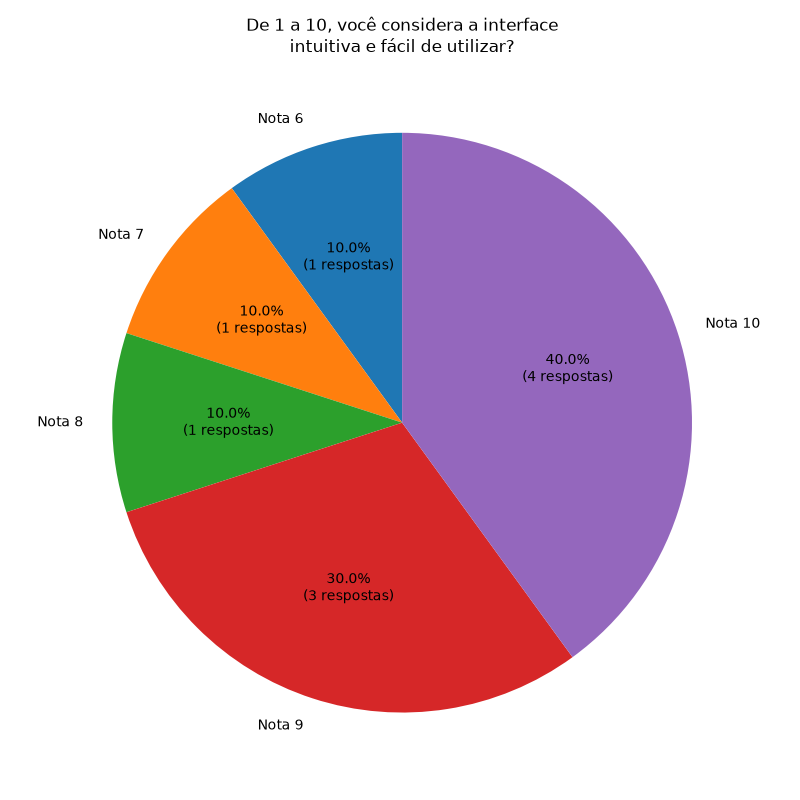
\includegraphics[width=0.9\linewidth]{images/interface_eval.png}
        \caption{Avaliação da usabilidade da interface}
        \label{fig:interface_eval}
    \end{figure}
    A Figura~\ref{fig:interface_eval} mostra que a interface foi em geral bem avaliada pelos participantes. As principais críticas envolveram:
    \begin{itemize}
        \item O contraste entre a fonte e a cor dos botões; 
        \item A notação presente nas alternativas, que dificultava a resolução da questão;
        \item O resultado da questão, que poderia ser apresentado logo após a submissão da resposta para saber se a resposta está correta 
    \end{itemize}


\subsection{Módulos mais difíceis}
    \begin{table}[H]
        \centering
        \caption{Módulos considerados mais difíceis pelos participantes}
        \label{tab:hardest_modules}
        \small
        \begin{tabular}{>{\centering\arraybackslash}m{3cm} >{\centering\arraybackslash}m{3cm} >{\centering\arraybackslash}m{8cm}}
\toprule
Módulo & Quantidade de participantes & Motivos \\
\midrule
Reconhecimento & 2 & \begin{itemize}\item Dificuldade em decorar as peças\item Explicações repetitivas e pouco úteis\end{itemize} \\\midrule
Movimento 1 & 0 & — \\\midrule
Movimento 2 & 1 & \begin{itemize}\item Dificuldade em diferenciar peças com movimentos semelhantes, principalmente as promovidas\end{itemize} \\\midrule
Promoção & 2 & \begin{itemize}\item Dificuldade em verificar todas alternativas apenas com a notação utilizada\item Explicações da IA insuficientes para compreender o conceito trabalhado\end{itemize} \\\midrule
Drop & 1 & \begin{itemize}\item Explicações da IA insuficientes para compreender o conceito trabalhado\end{itemize} \\\midrule
Xeque-mate & 4 & \begin{itemize}\item Maior dificuldade em analisar as alternativas e aplicar o raciocínio lógico\end{itemize} \\
\bottomrule
\end{tabular}


    \end{table}
 
\subsection{Progressão dos módulos}
A progressão dos módulos foi avaliada positivamente por 90\% dos participantes. Entre as justificativas apresentadas, 
destacaram-se a evolução gradual do nível de dificuldade e a construção de uma base de conhecimento, começando pelo 
reconhecimento das peças e seus movimentos antes de abordar mecânicas mais complexas, como promoção, drop e xeque-mate. 
Também foi mencionado que essa organização facilita a assimilação dos conceitos.

O participante restante não expressou uma avaliação direta sobre a progressão, mas apontou a ausência de um módulo 
introdutório que apresentasse as regras gerais do shogi, incluindo a disposição inicial das peças e o objetivo do jogo. 

\subsection{Quantidade de exercícios}
A quantidade de exercícios por lista foi considerada ideal por 80\% dos participantes, destacando que com isso foi possível
fixar melhor o conteúdo aprendido e revisar conceitos anteriores. Por outro lado, a principal crítica feita ao tamanho das listas
foi a repetitividade das questões, que, associada à ausência de explicações mais lúdicas, tornou a experiência de aprendizado menos 
dinâmica e as listas excessivamente longas.

\subsection{Compreensão dos fundamentos}
Todos os participantes consideraram que conseguiram aprender, ao menos parcialmente, os fundamentos básicos do shogi propostos pelo sistema. 
Entre as justificativas, destacaram-se a organização do conteúdo em módulos e a repetição dos exercícios, que contribuíram para a memorização 
das peças e de seus movimentos. Também foi mencionada a facilidade proporcionada pelas semelhanças com o xadrez e, em um caso, pelo conhecimento
prévio dos kanjis.

Por outro lado, alguns participantes relataram dificuldades na compreensão de conceitos específicos, principalmente as regras de promoção e drop. 
Além disso, houve críticas à qualidade das explicações fornecidas pela IA, consideradas insuficientes para esclarecer determinados erros, o que levou 
alguns participantes a recorrerem a materiais externos para complementar o aprendizado.

\subsection{Clareza e contribuição das explicações}
    \begin{figure}[H]
        \centering
        \begin{subfigure}{0.48\textwidth}
            \centering
            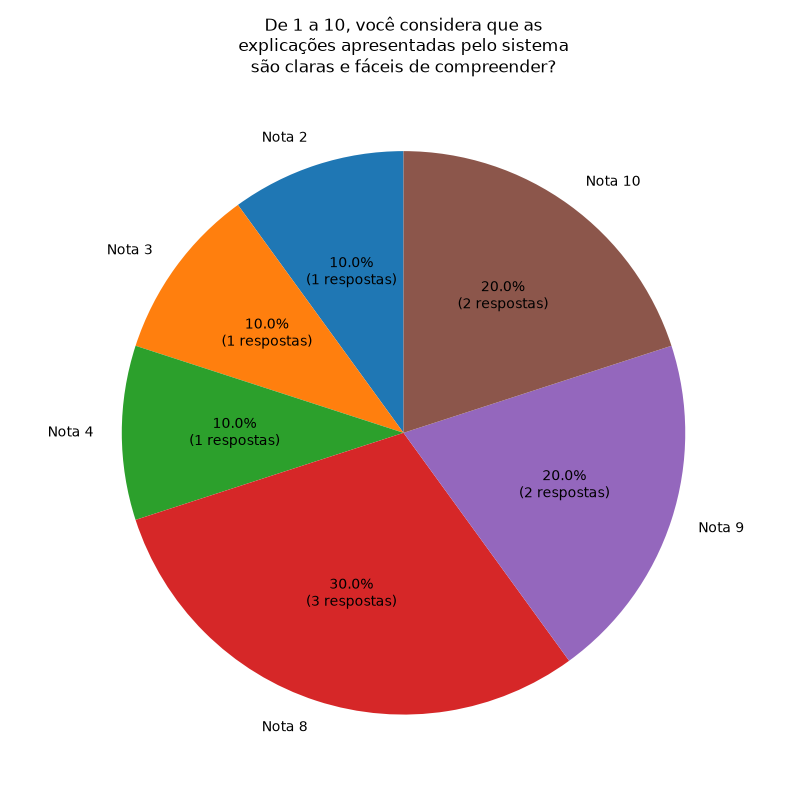
\includegraphics[width=\linewidth]{images/explanation_clarity_eval.png}
            \caption{Clareza das explicações}
            \label{fig:explanation_clarity_eval}
        \end{subfigure}
        \hfill
        \begin{subfigure}{0.48\textwidth}
            \centering
            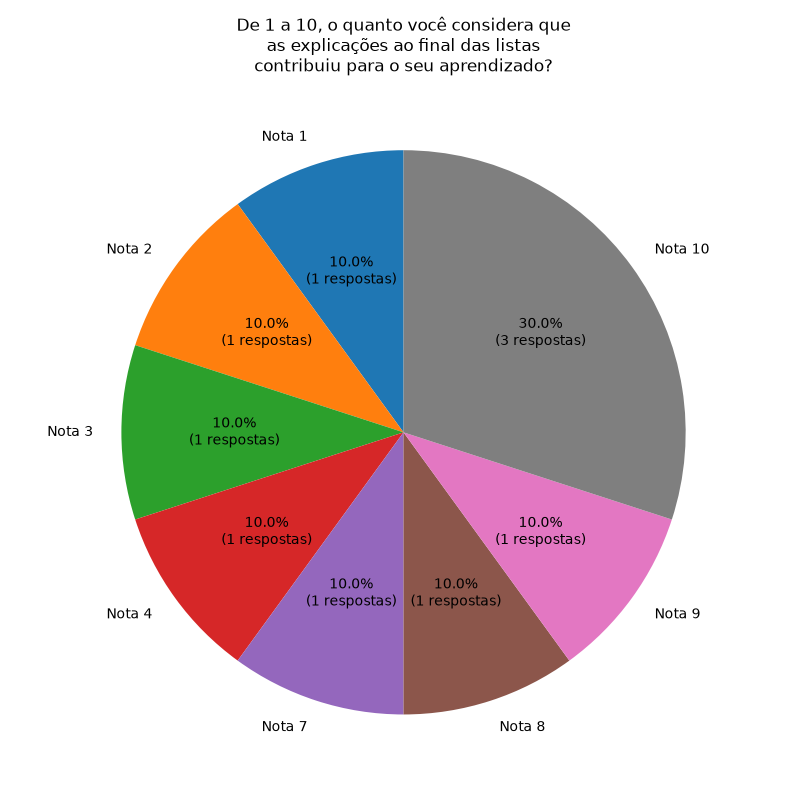
\includegraphics[width=\linewidth]{images/explanation_contribution_eval.png}
            \caption{Contribuição para o aprendizado}
            \label{fig:explanation_contribution_eval}
        \end{subfigure}
        \caption{Avaliação das explicações apresentadas pelo sistema}
        \label{fig:explanation_eval}
    \end{figure}

Conforme apresentado na Figura~\ref{fig:explanation_clarity_eval}, a clareza das explicações foi majoritariamente avaliada de forma positiva. 
Entretanto, essa percepção não se refletiu necessariamente na contribuição para o aprendizado, conforme observado na Figura~\ref{fig:explanation_contribution_eval}, 
cujas avaliações apresentaram maior variação.

As justificativas indicam que, embora as explicações tenham auxiliado alguns participantes a compreender os erros cometidos e consolidar os conceitos trabalhados, 
em determinadas situações foram consideradas vagas, confusas ou insuficientes para esclarecer o raciocínio por trás da resposta correta. Essa limitação também foi 
apontada entre as dificuldades relatadas na Tabela~\ref{tab:hardest_modules}.

Além disso, um participante destacou que a ausência de explicações para respostas corretas também pode prejudicar o aprendizado. Isso ocorre porque, ao acertar 
uma questão por eliminação ou tentativa, o usuário pode deixar de compreender o conceito envolvido, uma vez que não recebe uma explicação que justifique a alternativa selecionada.



\subsection{Sugestões de melhorias}

Entre os principais pontos de melhoria identificados pelos participantes, destacaram-se a inclusão de um módulo introdutório para apresentar os conceitos e as regras gerais 
do shogi antes do início das atividades e a distribuição dos exercícios entre as diferentes peças, especialmente as promovidas, já discutida na Seção~\ref{sec:users_performances}. 
Também foram sugeridas melhorias na visualização das peças e de seus movimentos no tabuleiro, de modo a facilitar a identificação das alternativas e reduzir a dependência da 
notação utilizada.

Além disso, alguns participantes apontaram a necessidade de diversificar os exercícios, reduzindo sua repetitividade e incluindo questões mais desafiadoras, assim como introduzir 
elementos lúdicos que incentivem a continuidade do aprendizado. Outras sugestões envolveram a disponibilização de feedback imediato após o envio das respostas e o aprimoramento das 
explicações geradas pela IA, para que apresentem justificativas mais contextualizadas e auxiliem na compreensão dos erros cometidos. Por fim, foi sugerida a inclusão de um módulo de 
prática interativa, permitindo que os usuários joguem partidas e recebam orientações sobre os movimentos possíveis.